The symbol of the lumped and Dirichled variants of BDDC are given by the symbol of the subassembled inverse and the respective injection operators.

\begin{definition}[Symbol of Lumped Balancing Domain Decomposition by Constraints]
The symbol of the lumped BDDC preconditioner is given by
\begin{equation}
\tilde{\mathbf{M}}^{-1}_1 = \tilde{\mathbf{R}}^T_1 \tilde{\hat{{\color{burgundy}\mathbf{A}}}}^{-1} \tilde{\mathbf{R}}_1
\end{equation}
where $\tilde{\mathbf{R}}_1$ is the symbol of the scaled injection operator, given by Definition \ref{def:scaled_injection_symbol}, and $\tilde{\hat{{\color{burgundy}\mathbf{A}}}}^{-1}$ is the symbol of the inverse of the subassembled problem, given by Definition \ref{def:subassembled_symbol}. 
\label{def:lumped_bddc_symbol}
\end{definition}

\begin{figure}[!ht]
  \centering
  \subfloat[Low-Order Lumped BDDC]{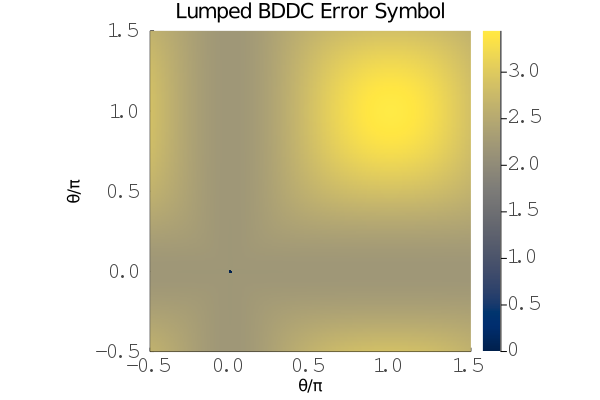
\includegraphics[width=0.48\textwidth]{../img/lumpedBDDCLowOrder}\label{fig:lumped_bddc_low_order}}
  \hfill
  \subfloat[High-Order Lumped BDDC]{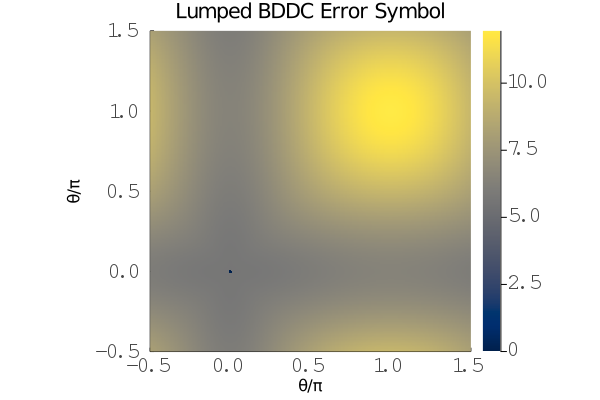
\includegraphics[width=0.48\textwidth]{../img/lumpedBDDCHighOrder}\label{fig:lumped_bddc_high_order}}
  \caption{Lumped BDDC Error Symbol}
\end{figure}

In Figure \ref{fig:lumped_bddc_low_order} we see the spectral radius of the symbol of the error operator of lumped BDDC for the scalar diffusion operator on a subdomain consisting of $16$ linear $H^1$ Lagrange finite elements.
In Figure \ref{fig:lumped_bddc_high_order} we see the spectral radius of the symbol of the error operator of lumped BDDC for the scalar diffusion operator on a subdomain consisting of a single finite element with a $4$th degree $H^1$ Lagrange basis.
We can see that lumped BDDC is significantly less effective on the subdomain consisting of a single high-order element.

\begin{definition}[Symbol of Dirichlet Balancing Domain Decomposition by Constraints]
The symbol of the Dirichlet BDDC preconditioner is given by
\begin{equation}
\tilde{\mathbf{M}}^{-1}_2 = \tilde{\mathbf{R}}^T_2 \tilde{\hat{{\color{burgundy}\mathbf{A}}}}^{-1} \tilde{\mathbf{R}}_2
\end{equation}
where $\tilde{\mathbf{R}}_2$ is the symbol of the harmonic injection operator, given by Definition \ref{def:harmonic_injection_symbol}, and $\tilde{\hat{{\color{burgundy}\mathbf{A}}}}^{-1}$ is the symbol of the inverse of the subassembled problem, given by Definition \ref{def:subassembled_symbol}. 
\label{def:dirichlet_bddc_symbol}
\end{definition}

\begin{figure}[!ht]
  \centering
  \subfloat[Low-Order Dirichlet BDDC]{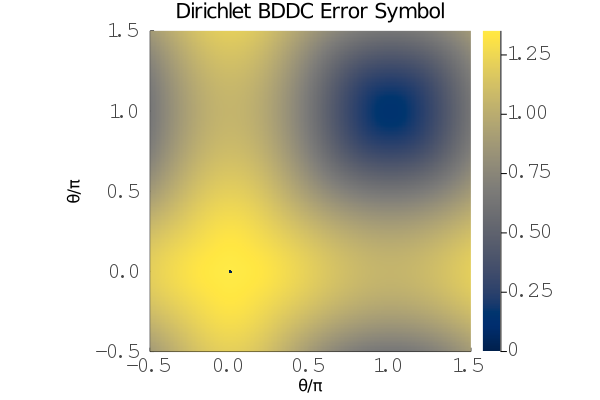
\includegraphics[width=0.48\textwidth]{../img/DirichletBDDCLowOrder}\label{fig:dirichlet_bddc_low_order}}
  \hfill
  \subfloat[High-Order Dirichlet BDDC]{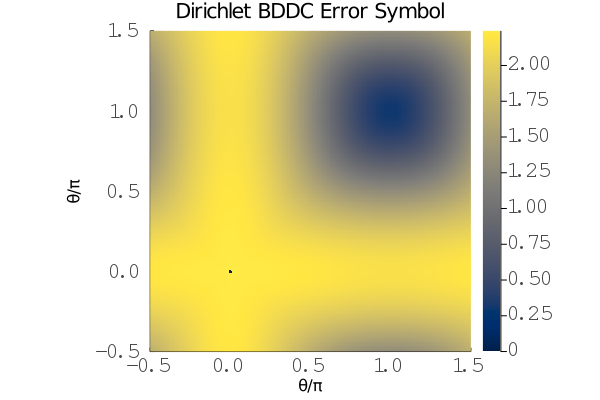
\includegraphics[width=0.48\textwidth]{../img/DirichletBDDCHighOrder}\label{fig:dirichlet_bddc_high_order}}
  \caption{Dirichlet BDDC Error Symbol}
\end{figure}

In Figure \ref{fig:dirichlet_bddc_low_order} we see the spectral radius of the symbol of the error operator of Dirichlet BDDC for the scalar diffusion operator on a subdomain consisting of $16$ linear $H^1$ Lagrange finite elements.
In Figure \ref{fig:dirichlet_bddc_high_order} we see the spectral radius of the symbol of the error operator of Dirichlet BDDC for the scalar diffusion operator on a subdomain consisting of a single finite element with a $4$th degree $H^1$ Lagrange basis.
We can see that Dirichlet BDDC is less effective on the subdomain consisting of a single high-order element, but the effect is not as pronounced as with lumped BDDC.
